\documentclass[12pt]{article}%
\usepackage{amsfonts}
\usepackage{fancyhdr}
\usepackage{comment}
\usepackage[a4paper, top=2.5cm, bottom=2.5cm, left=2.2cm, right=2.2cm]%
{geometry}
\usepackage{times}
\usepackage{amsmath}
\usepackage{changepage}
\usepackage{stfloats}
\usepackage{amssymb}
\usepackage{graphicx}
\usepackage{indentfirst}
\setlength{\parindent}{2em}
\setcounter{MaxMatrixCols}{30}
\newtheorem{theorem}{Theorem}
\newtheorem{acknowledgement}[theorem]{Acknowledgement}
\newtheorem{algorithm}[theorem]{Algorithm}
\newtheorem{axiom}{Axiom}
\newtheorem{case}[theorem]{Case}
\newtheorem{claim}[theorem]{Claim}
\newtheorem{conclusion}[theorem]{Conclusion}
\newtheorem{condition}[theorem]{Condition}
\newtheorem{conjecture}[theorem]{Conjecture}
\newtheorem{corollary}[theorem]{Corollary}
\newtheorem{criterion}[theorem]{Criterion}
\newtheorem{definition}[theorem]{Definition}
\newtheorem{example}[theorem]{Example}
\newtheorem{exercise}[theorem]{Exercise}
\newtheorem{lemma}[theorem]{Lemma}
\newtheorem{notation}[theorem]{Notation}
\newtheorem{problem}[theorem]{Problem}
\newtheorem{proposition}[theorem]{Proposition}
\newtheorem{remark}[theorem]{Remark}
\newtheorem{solution}[theorem]{Solution}
\newtheorem{summary}[theorem]{Summary}
\newenvironment{proof}[1][Proof]{\textbf{#1.} }{\ \rule{0.5em}{0.5em}}

\usepackage{mathtools}

\newcommand{\Q}{\mathbb{Q}}
\newcommand{\R}{\mathbb{R}}
\newcommand{\C}{\mathbb{C}}
\newcommand{\Z}{\mathbb{Z}}

\begin{document}

\title{MATH2040C Homework 6}
\author{ZHENG Weijia (William, 1155124322)}
\date{April 9, 2021}
\maketitle



\section{Section 6.1, Q8}

\begin{figure}[htp]
    \centering % 图片居中
    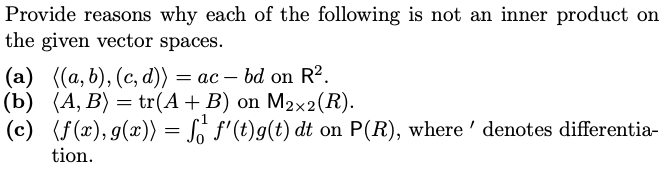
\includegraphics[width = 16cm]{img/Q1.png}
    \caption{The caption of this figure.}
    \label{fig:figure1label}
    \end{figure}


Let $w=\begin{pmatrix}2&4\\4&3\end{pmatrix}.$ Note that $w \in W$, because $w$ is symmetric.

Note that $T(w)=\begin{pmatrix}0&1\\1&0\end{pmatrix}\begin{pmatrix}2&4\\4&3\end{pmatrix}=\begin{pmatrix}4&3\\2&4\end{pmatrix},$ which is not symmetric, hence not belongs to $W$.

Therefore, by definition, $W$ is not a T-invariant subspace of $V.$

Done.



\end{document}
